\section{Vetores}

\subsection*{Plano Cartesiano}
\begin{frame}[label=vetores]{O conjunto $\R^2$}

Denotamos por   $\R^2$ o conjunto formado pelos {\color{blue}pares ordenados} $(x,y)$ tais $x$ $y$ são números reais. O número $x$ chama-se {\color{blue}primeira coordenada ou abcissa} e o número $y$ chama-se {\color{blue}segunda coordenada ou ordenada}. 
\medskip

Podemos representar geometricamente os elementos de $\R^2$ usando um {\color{blue}sistema de coordenadas cartesianas}, que consiste em um plano com um par de eixos perpendiculares $OX$ e $OY$ e que tem a mesma origem.

\begin{exe}
Em um plano, fixado um sistema de coordenadas cartesianas, represente:
\begin{enumerate}
\item Os pontos $P=(1,0)$, $Q=(2,1)$ e $R=(-3,-2)$.
\item Os conjuntos $A=\{(x,y)\in \R^2;\ x=1\}$ e $B=\{(x,y)\in \R^2;\ x=y\}$.
\end{enumerate}
\end{exe}

\end{frame}

\subsection*{Espaços Vetoriais}

\begin{frame}[label=vetores]{Espaços Vetoriais Reais}

Um {\color{blue}espaço vetorial real} $V$ é um conjunto, cujos elementos são chamados {\color{blue} vetores}, no qual estão definidas duas operações:

\begin{itemize}
\item A {\color{blue} adição}, que a cada par de vetores $\vec{u}$,$\vec{v}\in V$ faz corresponder um novo vetor $\vec{u}+\vec{v}$, chamado {\color{blue}vetor soma} de $\vec{u}$ e $\vec{v}$.

\item A {\color{blue} multiplicação por escalar}, que a cada número $\alpha\in \R$ e a cada vetor $\vec{v}\in V$ faz corresponder um vetor $\alpha \vec{v}$, chamado {\color{blue}produto de $\alpha$ por $\vec{v}$}.
\end{itemize}
Além disso, essas operações devem satisfazer, para quaisquer $\vec{u},\vec{v},\vec{w}\in V$ e $\alpha,\beta \in \R$, as seguintes condições:
%\begin{enumerate}
%\item $\vec{u}+\vec{v}=\vec{v}+\vec{u}$ (comutatividade)
%\item $(\vec{u}+\vec{v})+\vec{w}=\vec{u}+(\vec{v}+\vec{w})$ (associatividade)
%\item Existe um vetor $\vec{0}\in V$, chamado {\color{blue}vetor nulo}, tal que
%\[\vec{u}+\vec{0}=\vec{u} \text{ para todo } \vec{u}\in V.\]
%\end{enumerate}
\end{frame}


\begin{frame}[label=vetores]{Espaços Vetoriais Reais}

\begin{enumerate}

\item $\vec{u}+\vec{v}\in V$. (fechamento em relação à adição)
\item $\vec{u}+\vec{v}=\vec{v}+\vec{u}$ (comutatividade)
\item $(\vec{u}+\vec{v})+\vec{w}=\vec{u}+(\vec{v}+\vec{w})$ (associatividade)
\item Existe um vetor $\vec{0}\in V$, chamado {\color{blue}vetor nulo}, tal que
\[\vec{u}+\vec{0}=\vec{u} \text{ para todo } \vec{u}\in V.\]

\item Para cada $\vec{v}\in V$, existe um vetor $\vec{-v}\in E$, chamado {\color{blue}inverso aditivo}, ou {\color{blue}simétrico} de $\vec{v}$, tal que
\[-\vec{v}+\vec{v}=\vec{0}.\]

\item $\alpha \vec{v}\in V$. (fechamento em relação à multiplicação por escalar)

\item $(\alpha+\beta)\vec{v}=\alpha \vec{v}+\beta \vec{v}$ e $\alpha(\vec{u}+\vec{v})=\alpha\vec{v}+\alpha\vec{v}$. (distributividade)

\item $1\cdot \vec{v}=\vec{v}$.
\end{enumerate}
\end{frame}

\subsection*{Vetores no $\R^2$}

\begin{frame}[label=vetores]{O Espaço Vetorial $\R^2$}

O conjunto $\R^2$ torna-se um espaço vetorial quando o munimos com as seguintes  operações: Se $\vec{u}=(u_1,u_2)$,  $\vec{v}=(v_1,v_2)$ e $\alpha\in \R$ então
\[\vec{u}+\vec{v}=(u_1+v_1,u_2+v_2),\]
\[\alpha \vec{v}=(\alpha v_1,\alpha v_2).\]
Neste caso, o {\color{blue}vetor nulo} é $\vec{0}=(0,0)$ e o {\color{blue}simétrico} de $\vec{v}$ é  $-\vec{v}=(-v_1,-v_2)$.


\end{frame}


\begin{frame}[label=vetores]{Representação Geométrica}

Representamos um vetor $\vec{u}=(u_1,u_2)$ de $\R^2$ usando um {\color{blue}segmento orientado} com {\color{blue}ponto inicial} na origem do sistema de coordenadas e {\color{blue}extremidade} no ponto $P=(u_1,u_2)$.

\begin{center}
		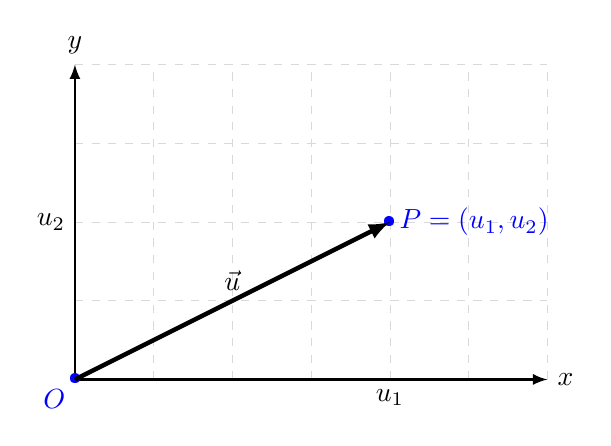
\begin{tikzpicture}[scale=1]
		\tikzset{>=latex}
	\draw[help lines, color=gray!30, dashed] (0,0) grid (6,4);
	\draw[->,thick] (0,0)--(6,0) node[right]{$x$};
	\draw[->,thick] (0,0)--(0,4) node[above]{$y$};
%	\foreach \i in {1,...,7}
%	\node[below,scale=0.7] at (\i,0) {$\i$};
%	\foreach \i in {1,...,4}
%	\node[left,scale=0.7] at (0,\i) {$\i$};


\coordinate (O) at (0,0);
\coordinate (E) at (4,2);
\node[left,scale=1] at (0,2) {$u_2$};
\node[below,scale=1] at (4,0) {$u_1$};

	\node[blue] at (O) {\textbullet};
\node[blue,below left] at (O) {$O$};
	
\node[blue] at (E) {\textbullet};
\node[blue,right] at (E) {$P=(u_1,u_2)$};

\node[above] at (2,1) {$\vec{u}$};

\draw[->,ultra thick] (O) -- (E);
	
	\end{tikzpicture}
\end{center}

Neste caso, escrevemos $\vec{u}=\overrightarrow{OP}$. 

\end{frame}

\subsection*{Norma de um vetor}
\begin{frame}[label=vetores]{Norma de um vetor}

O {\color{blue}comprimento} de vetor $\vec{u}$, também chamado de {\color{blue}norma}, é dado por:

\begin{center}
\begin{minipage}{0.5\textwidth}
\begin{block}{}
\[\|\vec{u}\|=\sqrt{u_1^2+u_2^2}.\]
\end{block}
\end{minipage}
\end{center}


\begin{exe}
Represente no plano o vetor $\vec{u}=(1,1)$ e calcule seu comprimento.
\end{exe}
\end{frame}

\subsection*{Lei do Paralelogramo}

\begin{frame}[label=vetores]{Representação Geométrica da Soma}

Dados dois vetores ${\color{red}\vec{u}=(u_1,u_2)}$ e ${\color{blue}\vec{v}=(v_1,v_2)}$ de $\R^2$  o vetor soma 
\[\vec{u}+\vec{v}=(u_1+v_1,u_2+v_2)\]
é obtido pela chamada {\color{blue}lei do paralelogramo}.

\begin{center}
		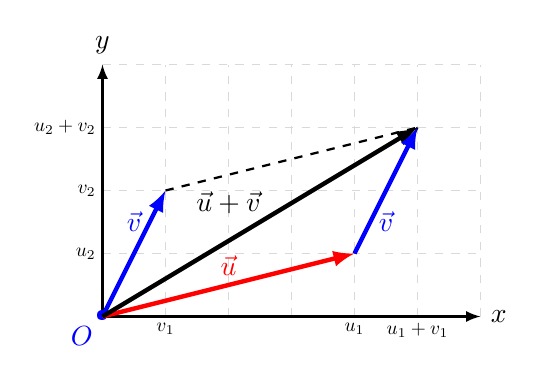
\begin{tikzpicture}[scale=0.8]
		\tikzset{>=latex}
	\draw[help lines, color=gray!30, dashed] (0,0) grid (6,4);
	\draw[->,thick] (0,0)--(6,0) node[right]{$x$};
	\draw[->,thick] (0,0)--(0,4) node[above]{$y$};



\coordinate (O) at (0,0);
\coordinate (A) at (1,2);
\coordinate (B) at (4,1);
\coordinate (C) at (5,3);
\node[left,scale=.7] at (0,1) {$u_2$};
\node[below,scale=.7] at (4,0) {$u_1$};

\node[left,scale=0.7] at (0,2) {$v_2$};
\node[below,scale=0.7] at (1,0) {$v_1$};

\node[left,scale=.7] at (0,3) {$u_2+v_2$};
\node[below,scale=.7] at (5,0) {$u_1+v_1$};

\node at (2,0.8) {${\color{red}\vec{u}}$};
\node<1> at (0.5,1.5) {${\color{blue}\vec{v}}$};
\node<2> at (4.5,1.5) {${\color{blue}\vec{v}}$};
\node at (2,1.8) {$\vec{u}+\vec{v}$};
\node[blue] at (O) {\textbullet};
\node[blue,below left] at (O) {$O$};
	
\draw<1>[->,ultra thick,blue] (O) -- (A);
\draw[->,ultra thick,red] (O) -- (B);
\draw[->,ultra thick] (O) -- (C);

\draw<1>[dashed,thick] (A) -- (C);
\draw<1>[dashed,thick] (B) -- (C);
\draw<2>[->,ultra thick,blue] (B) -- (C);
	
	\end{tikzpicture}
\end{center}



\end{frame}

\subsection*{Coordenadas de um Vetor}

\begin{frame}[label=vetores]

Dizemos que um segmento de reta orientado {\color{red}$\overrightarrow{AB}$} também representa um vetor ${\color{blue}\vec{u}}$ quando os dois têm mesmo {\color{blue}comprimento, direção e sentido}. Neste caso, escrevemos ${\color{blue}\vec{u}}={\color{red}\overrightarrow{AB}}$.



\begin{center}
		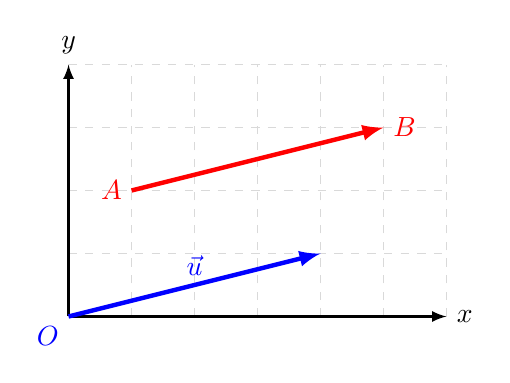
\begin{tikzpicture}[scale=0.8]
		\tikzset{>=latex}
	\draw[help lines, color=gray!30, dashed] (0,0) grid (6,4);
	\draw[->,thick] (0,0)--(6,0) node[right]{$x$};
	\draw[->,thick] (0,0)--(0,4) node[above]{$y$};



\coordinate (O) at (0,0);
\coordinate (A) at (1,2);
\coordinate (B) at (4,1);
\coordinate (C) at (5,3);

\node at (2,0.8) {${\color{blue}\vec{u}}$};
\node[blue,below left] at (O) {$O$};
\node[red,left] at (A) {$A$};
\node[red,right] at (C) {$B$};
	
\draw<1>[->,ultra thick,blue] (O) -- (B);

\draw[->,ultra thick,red] (A) -- (C);
	\end{tikzpicture}
\end{center}

\begin{center}
\begin{minipage}{0.7\textwidth}
\begin{block}{}
Se {\color{red}$A=(a_1,a_2)$} e {\color{red}$B=(b_1,b_2)$} então
\[{\color{red}\overrightarrow{AB}}={\color{blue}\vec{u}=(b_1-a_1,b_2-a_2)}.\]
\end{block}
\end{minipage}
\end{center}

\end{frame}

\begin{frame}[label=vetores]
De uma forma geral temos que 
\begin{center}
\begin{minipage}{0.7\textwidth}
\begin{block}{}
\[\|{\color{red}\overrightarrow{AB}}\|=\sqrt{{\color{blue}(b_1-a_1)^2+(b_2-a_2)^2}}.\]
\end{block}
\end{minipage}
\end{center}


\begin{exe}
Dados $A=(1,1)$, $B=(2,2)$, $C=(-1,0)$ e $D=(0,1)$. Mostre que $\overrightarrow{AB}=\overrightarrow{CD}$ e calcule sua norma.
\end{exe}

\end{frame}




\begin{frame}[label=vetores]


Basta usar a lei do paralelogramo. 

\begin{center}
		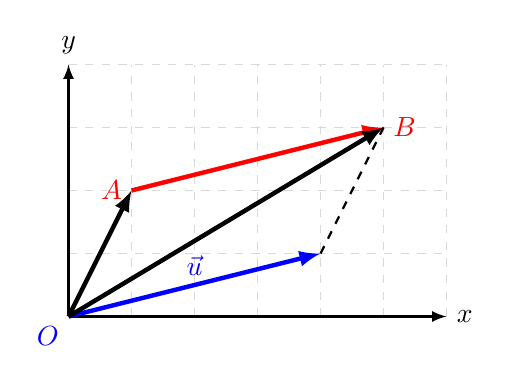
\begin{tikzpicture}[scale=0.8]
		\tikzset{>=latex}
	\draw[help lines, color=gray!30, dashed] (0,0) grid (6,4);
	\draw[->,thick] (0,0)--(6,0) node[right]{$x$};
	\draw[->,thick] (0,0)--(0,4) node[above]{$y$};



\coordinate (O) at (0,0);
\coordinate (A) at (1,2);
\coordinate (B) at (4,1);
\coordinate (C) at (5,3);

\node at (2,0.8) {${\color{blue}\vec{u}}$};
\node[blue,below left] at (O) {$O$};
\node[red,left] at (A) {$A$};
\node[red,right] at (C) {$B$};
	
\draw<1>[->,ultra thick,blue] (O) -- (B);

\draw[->,ultra thick,red] (A) -- (C);
\draw[->,ultra thick] (O) -- (A);
\draw[->,ultra thick] (O) -- (C);
\draw[dashed,thick] (B) -- (C);
	\end{tikzpicture}
\end{center}



Se {\color{blue}$\vec{u}=(x,y)$}, então
\[\overrightarrow{OA}+{\color{blue}\vec{u}}=\overrightarrow{OB}\Rightarrow (a_1+{\color{blue}x},a_2+{\color{blue}y})=(b_1,b_2),\]
donde
\[\begin{cases}
{\color{blue}x}=b_1-a_1\\
{\color{blue}y}=b_2-a_2.
\end{cases}\]

\end{frame}


\begin{frame}[label=vetores]

Em resumo, dados $A=(a_1,a_2)$ e $B=(b_1,b_2)$, escrevemos
\[\overrightarrow{AB}=(b_1-a_1,b_2-a_2).\]

Além disso, se tomarmos vetores $\overrightarrow{AB}$ e $\overrightarrow{BC}$, podemos escrever a soma da seguinte forma:
\[{\color{blue}\overrightarrow{AB}}+{\color{red}\overrightarrow{BC}}=\overrightarrow{AC}.\]

\begin{center}
		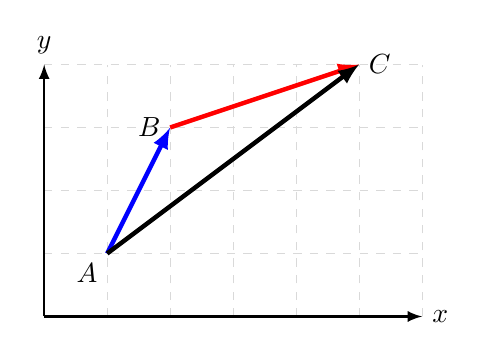
\begin{tikzpicture}[scale=0.8]
		\tikzset{>=latex}
	\draw[help lines, color=gray!30, dashed] (0,0) grid (6,4);
	\draw[->,thick] (0,0)--(6,0) node[right]{$x$};
	\draw[->,thick] (0,0)--(0,4) node[above]{$y$};



\coordinate (O) at (1,1);
\coordinate (A) at (2,3);
\coordinate (B) at (4,1);
\coordinate (C) at (5,4);

\node[below left] at (O) {$A$};
\node[left] at (A) {$B$};
\node[right] at (C) {$C$};
	
\draw<1>[->,ultra thick,blue] (O) -- (A);

\draw[->,ultra thick,red] (A) -- (C);
\draw[->,ultra thick] (O) -- (C);

	\end{tikzpicture}
\end{center}


\end{frame}



\begin{frame}[label=vetores]


\begin{casa}
Localize os pontos $A=(1,1)$, $B=(-3,0)$, $C=(4,1)$, $D=(2,-3)$ e $E=(3,-2)$ no plano cartesiano. Determine as coordenadas dos vetores abaixo e esboce um de seus representantes.
			
\begin{enumerate}
\item $\vt{u}=\vt{AB}+\vt{AC}+\vt{AD}$
				
\item $\vec{v}=2(\vt{BC}-\vt{EC})+3\vt{EF}-2\vt{AD}$
	
\end{enumerate}
\end{casa}

\end{frame}


\begin{frame}[label=vetores]{Representação Geométrica do Produto por Escalar}
Geometricamente, a {\color{blue}multiplicação escalar} estica, contrai ou troca de sentido um vetor.


	\begin{center}
		\begin{tikzpicture}
		\tikzset{>=latex}
%			
	\onslide<2->{\draw<1->[->, thick,blue] (0,0) -- (4,1);}
\onslide<2->{	\node[above ,blue] at (4,1) {$2\vect{u}$};}
\onslide<1->{\draw<1->[->,ultra thick] (0,0) -- (2,.5);
		\node[above ] at (2,0.5) {$\vect{u}$};}

	\onslide<3->{\draw[->, thick,red] (0,0) -- (-4,-1);}
	\onslide<3->{\node[above left ,red] at (-4,-1) {$-2\vect{u}$};}
	\onslide<4->{\draw[->, ultra thick,green] (0,0) -- (1,.25);
	\node[above,green ] at (1,0.25) {$\frac{1}{2}\vect{u}$};	}
		\end{tikzpicture}
	\end{center}

\end{frame}

\subsection*{Vetores no $\R^3$}
\begin{frame}[label=vetores]{O conjunto  $\R^3$}
Denotamos por   $\R^3$ o conjunto formado pelas {\color{blue}triplas ordenadas} $(x,y,z)$ tais $x$, $y$ e $z$ são números reais.
\medskip

Podemos representar geometricamente os elementos de $\R^3$ usando um {\color{blue}sistema de coordenadas cartesianas}, que consiste na escolha de três  eixos com a mesma origem, $OX$, $OY$ e $OZ$, mutuamente perpendiculares e que a orientação positiva é escolhida de acordo com a {\color{blue} regra da mão direita}.

\begin{center}
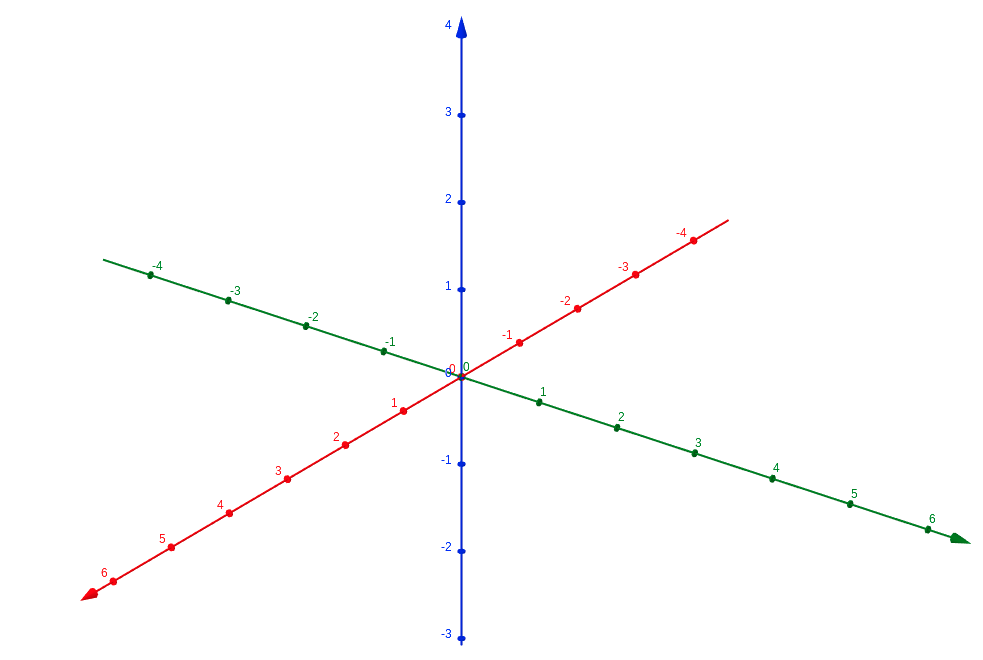
\includegraphics[scale=0.2]{figuras/eixos3d2.png}
\end{center}
\end{frame}


\begin{frame}[label=vetores]

\begin{exe}
\begin{enumerate}
\item Determine os pontos $(1,3,1)$ e $(3,-2,2)$ no sistema cartesiano.
\item Esboce o conjunto dos pontos que satisfazem a equação $z=3$.
\end{enumerate}
\end{exe}


\end{frame}


\begin{frame}[label=vetores]{Vetores no $\R^3$}
O conjunto $\R^3$ torna-se um espaço vetorial quando o munimos com as seguintes  operações: Se $\vec{u}=(u_1,u_2,u_3)$,  $\vec{v}=(v_1,v_2,v_2)$ e $\alpha\in \R$ então
\[\vec{u}+\vec{v}=(u_1+v_1,u_2+v_2,u_3+v_3),\]
\[\alpha \vec{v}=(\alpha v_1,\alpha v_2,\alpha v_3).\]
Neste caso, o {\color{blue}vetor nulo} é $\vec{0}=(0,0,0)$ e o {\color{blue}simétrico} de $\vec{v}$ é  $-\vec{v}=(-v_1,-v_2,-v_3)$.

\begin{center}
\begin{minipage}{0.7\textwidth}
\begin{block}{}
Se {\color{red}$A=(a_1,a_2,a_3)$} e {\color{red}$B=(b_1,b_2,b_3)$} então
\[{\color{red}\overrightarrow{AB}}={\color{blue}\vec{u}=(b_1-a_1,b_2-a_2,b_3-a_3)}.\]
\end{block}
\end{minipage}
\end{center}
\end{frame}


\begin{frame}[label=vetores]
Do mesmo modo,
\begin{center}
\begin{minipage}{0.7\textwidth}
\begin{block}{}
\[\|{\color{red}\overrightarrow{AB}}\|=\sqrt{{\color{blue}(b_1-a_1)^2+(b_2-a_2)^2 +(b_3-a_3)^2}}.\]
\end{block}
\end{minipage}
\end{center}


\begin{exe}
Dados $A=(0,3,1)$, $B=(2,3-1)$ e $C=(0,1,0)$ determine $2\vt{AB}+\vt{AC}$.
\end{exe}


\end{frame}

\subsection*{Vetores no $\R^n$}
\begin{frame}[label=vetores]{Vetores no $\R^n$}

De modo geral, denotamos por   $\R^n$ o conjunto formado pelas {\color{blue} $n$-uplas ordenadas} $(x_1,x_2,\ldots,x_n)$ tais $x_i\in \R$ para todo $i=1,2,\ldots,n$.
\medskip

O conjunto $\R^n$ torna-se um espaço vetorial quando o munimos com as seguintes  operações: Se $\vec{u}=(u_1,u_2,\ldots,u_n)$,  $\vec{v}=(v_1,v_2,\ldots,v_n)$ e $\alpha\in \R$ então
\[\vec{u}+\vec{v}=(u_1+v_1,u_2+v_2,\ldots,u_n+v_n),\]
\[\alpha \vec{v}=(\alpha v_1,\alpha v_2,\ldots,\alpha v_n).\]
Neste caso, o {\color{blue}vetor nulo} é $\vec{0}=(0,0,\ldots,0)$ e o {\color{blue}simétrico} de $\vec{v}$ é  $-\vec{v}=(-v_1,-v_2,\ldots,-v_n)$.

\begin{center}
\begin{minipage}{0.7\textwidth}
\begin{block}{}
Se {\color{red}$A=(a_1,a_2,\ldots,a_n)$} e {\color{red}$B=(b_1,b_2,\ldots,b_n)$} então
\[{\color{red}\overrightarrow{AB}}={\color{blue}\vec{u}=(b_1-a_1,b_2-a_2,\ldots,b_n-a_n)}.\]
\end{block}
\end{minipage}
\end{center}

\end{frame}

\begin{frame}[label=vetores]
De forma análoga, também definimos a {\color{blue} norma (ou comprimento)} de um vetor do $\R^n$ por
\begin{center}
\begin{minipage}{0.7\textwidth}
\begin{block}{}
Se {\color{blue}$\vec{u}=(u_1,u_2,\ldots,u_n)$} então
\[{\color{blue}\vec{u}=\sqrt{u_1^2+u_2^2+\ldots+u_n^2}}.\]
\end{block}
\end{minipage}
\end{center}

Um {\color{blue} vetor unitário} é um vetor que tem norma 1. Dado qualquer vetor não nulo $\vec{v}$, sempre podemos obter um {\color{blue}vetor unitário} $\vec{u}$ com mesmo sentido de $\vec{v}$, basta fazer
\[\vec{u}=\frac{1}{\|\vec{v}\|}\vec{v}.\]
Esse processo é chamada de {\color{blue} normalização} de $\vec{v}$. Alguns textos usam a notação $\hat{v}$ e o chamam de {\color{blue}versor}.


\end{frame}

\begin{frame}[label=vetores]


\begin{exe}
Normalize o vetor $\vec{v}=(2,-1,3)$.
\end{exe}


\begin{casa}
Normalize os vetores $\vec{u}=(1,\sqrt{2},\sqrt{3},0)$ e $\vec{v}=(4,-\sqrt{2},0,-5)$.
\end{casa}
\end{frame}

\begin{frame}[label=vetores]
Um nutricionista forneceu uma tabela que especifica a {\color{blue} quantidade mínima de cada tipo de vitamina que deve ser ingerida diariamente}.

\begin{center}

\begin{tabu}{|l|c|c|c|c|}
\hline
Tipo de vitamina & A & B & C & E\\ \hline
 Quantidade  mínima (mg) & 3 & 1.1 & 60 & 11\\ \hline
\end{tabu} 
\end{center}

Ele também forneceu uma tabela com a quantidade (em mg) de vitaminas em cada 100 gramas de 4 tipos de alimentos diferentes,
\begin{center}
\begin{tabu}{|c|c|c|c|c|}
\hline
& \multicolumn{4}{c|}{Alimento} \\ \hline
Vitamina & 1 & 2 & 3 & 4  \\ \hline
 \rowfont{\color{blue}} A &  0.140 & 0.580  & 0.150 & 0 \\ \hline
 \rowfont{\color{blue}} B &  0.08  & 0      & 1.30  & 0.08  \\ \hline
 \rowfont{\color{blue}} C &  0     & 0      & 26    & 38  \\ \hline
 \rowfont{\color{blue}} E & 1.60  & 0      & 6.90    & 0.2 \\ \hline
\end{tabu}
\end{center}

 Cada alimento é uma {\color{red}variável}, ou seja, 
\begin{center}
 $x_i$ representa a quantidade (em ``pacotes'' de 100g) do alimento $i$ que deve ser consumido diariamente, com $i=1,\ldots,4$. 
 \end{center}\bigskip

\end{frame}

\begin{frame}[label=vetores]
Com isso, se quisermos saber qual a quantidade de cada alimentos devemos consumir, para se ter a quantidade mínima de cada vitamina, devemos resolver o sistema:
\[
\begin{cases}
{\color{blue}0.14 } {\color{red}x_1}+ {\color{blue}0.58}{\color{red}x_2}+ {\color{blue}0.15}{\color{red}x_3}= 3,\\
{\color{blue}0.08}{\color{red}x_1}+{\color{blue}1.3}{\color{red}x_3}+{\color{blue}0.08}{\color{red}x_4}= 1.1,\\
{\color{blue}26}{\color{red}x_3}+{\color{blue}38}{\color{red}x_4}=  60,\\
{\color{blue}1.6}{\color{red}x_1}+{\color{blue}6.9}{\color{red}x_3}+{\color{blue}0.2}{\color{red}x_4}=  11,
\end{cases} 
\]
Usando a notação vetorial, temos:

\[
{\color{blue}
\begin{bmatrix}
0.14 \\ 0.08 \\ 0 \\ 1.60
\end{bmatrix}} {\color{red}x_1}+
{\color{blue}
\begin{bmatrix}
0.58 \\ 0 \\ 0 \\ 0
\end{bmatrix}} {\color{red}x_2}+
{\color{blue}
\begin{bmatrix}
0.150 \\ 1.30 \\ 26 \\ 6.90
\end{bmatrix}} {\color{red}x_3}+
{\color{blue}
\begin{bmatrix}
0\\ 0.08 \\ 38 \\ 0.2
\end{bmatrix}} {\color{red}x_4}=
\begin{bmatrix}
3 \\ 1.1\\ 60 \\ 11
\end{bmatrix}
\]
\end{frame}

\begin{frame}[label=vetores,fragile=singleslide]
\begin{pycode} 
import sympy as sp

x1,x2,x3,x4=sp.symbols('x_1 x_2 x_3 x_4',real=True)
X=sp.Matrix([x1,x2,x3,x4])
def pt(Y):
 return((Y[0],Y[1]))

v1=sp.Matrix([0.14,0.08,0,1.6])
v2=sp.Matrix([0.58,0,0,0])
v3=sp.Matrix([0.15,1.3,26,6.9])
v4=sp.Matrix([0,0.08,38,0.2])
B=sp.Matrix([3,1.1,60,11])

A=sp.Matrix.hstack(v1,v2,v3,v4)

AX=A*X
sol=sp.solve(sp.Eq(AX,B),(x1,x2,x3,x4))
\end{pycode} 
Aprenderemos mais à frente que este sistema tem a seguinte solução
\[x_1 \approx\pyl{sp.N(sol[x1],3)},\ x_2 \approx\pyl{sp.N(sol[x2],3)},\ x_3 \approx\pyl{sp.N(sol[x3],3)}\ \text{ e }\ x_4 \approx\pyl{sp.N(sol[x4],3)}.\]
Isto é, para se {\color{blue}ingerir a quantidade mínima de cada tipo de vitamina} devemos consumir:
\begin{center}

$\pyl{sp.N(sol[x1]*100,3)}$ gramas do alimento 1\\
$\pyl{sp.N(sol[x2]*100,3)}$ gramas do alimento 2\\
$\pyl{sp.N(sol[x3]*100,3)}$ gramas do alimento 3\\
$\pyl{sp.N(sol[x4]*100,3)}$ gramas do alimento 4
\end{center}
\end{frame}


\begin{frame}[label=vetores,fragile=singleslide]{Combinação Linear}

\begin{defin}
Um vetor $\vec{v}\in \R^n$ é uma {\color{blue} combinação linear} de vetores $\vec{v}_1, \vec{v}_2, \ldots, \vec{v}_k$ se existem escalares $\alpha_1,\alpha_2,\ldots, \alpha_k$ tais que
\[\vec{v}=\alpha_1\vec{v}_1+\alpha_2\vec{v}_2+\cdots +\alpha_k\vec{v}_k.\]
\end{defin}

\begin{pycode} 
import sympy as sp

x1,x2,x3,x4=sp.symbols('x_1 x_2 x_3 x_4',real=True)
X=sp.Matrix([x1,x2,x3,x4])
def pt(Y):
 return((Y[0],Y[1],Y[2],Y[3]))

v1=sp.Matrix([0.14,0.08,0,1.6])
v2=sp.Matrix([0.58,0,0,0])
v3=sp.Matrix([0.15,1.3,26,6.9])
v4=sp.Matrix([0,0.08,38,0.2])
B=sp.Matrix([3,1.1,60,11])
\end{pycode} 

No exemplo anterior, escrevemos  o vetor $\vec{v}=\pyl{B}$ como combinação linear dos vetores
\[\vec{v}_1=\pyl{v1},\ \vec{v}_2=\pyl{v2},\ \vec{v}_3=\pyl{v3},\ \text{ e } \vec{v}_4=\pyl{v4}. \]

\end{frame}
